\chapter{Results}

\section{Generation Time}

\begin{figure}[h]
	\centering
	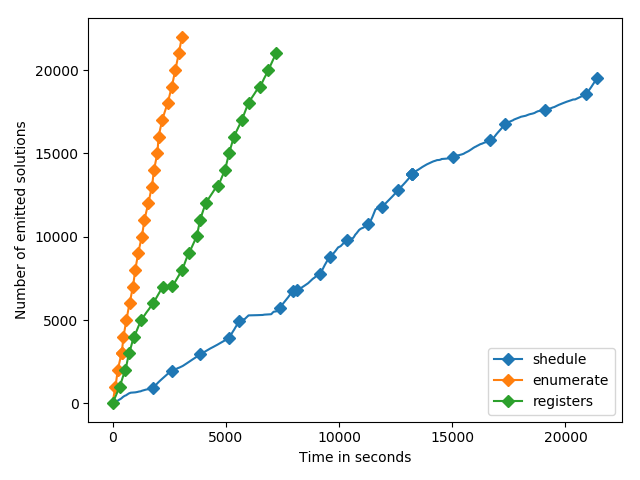
\includegraphics[width=\textwidth,height=0.5\textheight]{results/figures/generator_time}
	\caption{The execution time of the code generator at sampling rate 1000 (i.e 1000000 solutions for every function). Each marker represents the finished generation of a function.}
	\label{fig:time}
\end{figure}

\section{Cost}

The estimated cost of each program is shown in Figure \ref{fig:cost}. The dotted red line
shows the cost of the LLVM solution when calculated in the same manner.

\begin{figure}[h]
	\centering
	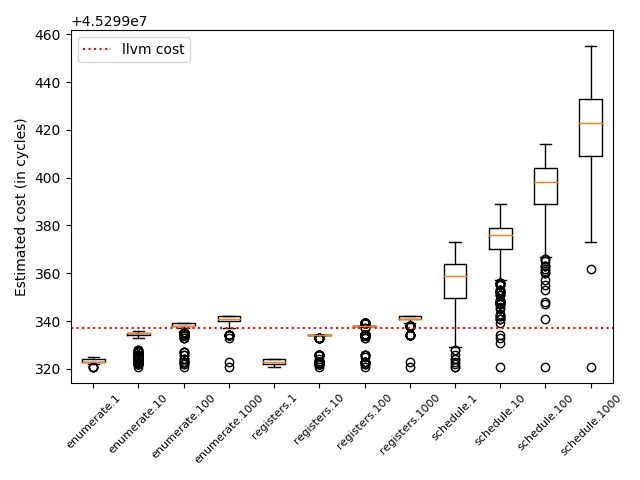
\includegraphics[width=\textwidth,height=0.5\textheight]{results/figures/cost}
	\caption{The cost distributions for every strategy and sampling rate. The cost of the LLVM solution is included for reference.}
	\label{fig:cost}
\end{figure}

All strategies perform better for lower sampling rates. As described in section
\ref{sec:performance}, this is expected. Enumerate and registers perform equally well and
for sampling sizes of 1 and 10 they have a lower cost than the LLVM solution. The schedule
strategy seems to incur a slight overhead compared to the LLVM solution for all sampling
rates.

\begin{table}[h]
		\centering
		\noindent\makebox[\textwidth]{%
			\begin{tabular}{rrrr}
\hline
   Sampling Rate &   Est. Cost (cycles) &   Difference (cycles) &   Overhead (\textperthousand) \\
\hline
               1 &             45299359 &                    22 &                      0.000486 \\
              10 &             45299376 &                    39 &                      0.000861 \\
             100 &             45299398 &                    61 &                      0.001347 \\
            1000 &             45299423 &                    86 &                      0.001898 \\
\hline
\end{tabular}
		}
		\caption{The cost of the different sampling rates for the schedule strategy compared to the LLVM solution.%
		The difference column is the difference between the median cost of the sampling rate and the cost of the LLVM solution.}
		\label{table:sched_cost}
\end{table}

Table \ref{table:sched_cost} shows the cost difference between the different sampling
rates for the schedule strategy compared to the cost of the LLVM program. The overhead of
the schedule strategy is negligible (note that the overhead column shows per mille). All
sampling rates have versions with a lower cost than the LLVM solution so if only a few
versions are necessary there is potential to limit the constraint solver to only find
those with lower cost than LLVM.

Interesting to note is that all strategies and sampling rates have found a solution with
an equally low cost. This is presumably the very first solution found; When no strategy
related constraints have been posted yet.

\section{Surviving Gadgets} 
\begin{figure}[htp]
	\centering
	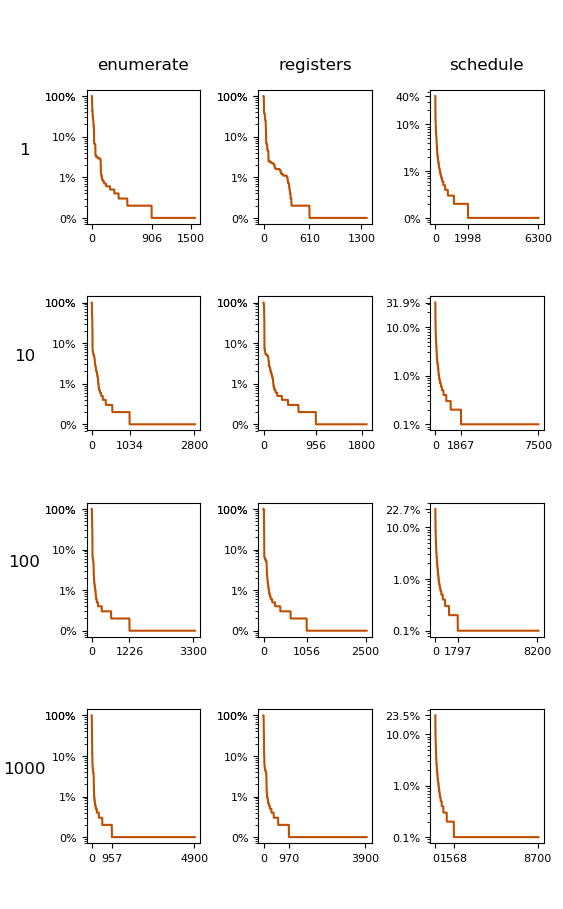
\includegraphics[width=\textwidth,height=\textheight]{results/figures/gadgets}
	\caption{The ratio of occurence for each gadget broken down by strategy and sampling rate.
Each bar shows the occurence ratio for one particular gadget.}
	\label{fig:gadgets}
\end{figure}

Figure \ref{fig:gadgets} shows the occurence ratio of each gadget for the different
strategies and sampling rates. There were around 21000 gadgets in total for every program
across all versions. The x-axis shows a gadget id and there is no definitive correlation
between the gadgets across strategies and sampling rates. I.e gadget 0 for the enumerate
strategy at sampling rate 1 is not necessarily the same gadget 0 as the registers strategy
at sampling rate 10.

As seen in figure \ref{fig:gadgets}, neither the enumeration nor the registers strategy
were particularly effective at breaking gadgets for any sampling rate. There is a slight
improvement for higher sampling rates but it is not particularly impressive even at
sampling rate 1000. There are still many gadgets that survives between versions.

Curiously, there seems to be little difference between sampling rate 10 and 100 for both
enumerate and registers. Sampling rate of 100 appears to be even worse at breaking gadgets
than sampling rate 10. This is surprising and there is no definitive explanation for it.
I suspect this is because.... ?

As mentioned, \textcite{large-scale-automated} found that randomizing the instruction
schedule broke on average more than 95\% gadgets with respect to the original, undiversifed
binary. This would then mean that on average less than 5\% of gadgets survive the
diversification process and are present in all versions, compared to our results where
\textit{no} gadget is present is all versions. In fact, no gadget is present in even
50\% of versions. The strategy is even more effective at higher sampling rates, which is
in accordance with the expected behaviour described in section \ref{sec:sampling_rate}.

\section{Conclusion and Future Work}

While both the enumerate and registers strategies showed great results in terms of cost,
neither of them were effective at breaking gadgets. With regards to both the gadget
breaking properties and estimated cost of the schedule strategy the hypothesis definitely
holds true. More gadgets are broken and the overhead with respect to the LLVM solution
is negligible.

For a more proper comparison of the systematic approach tests would have to be repeated
targeting the 86-64 architecture. As mentioned in Section \ref{sec:arch} Unison in its
current state does not support the x86-64 architecture. If or when Unison or a similar
tool implements support for the x86-64 architecture, or at the very least an architecture
with a complex instruction set, the experiment would have be repeated on that platform to
test whether or not the strategies are equally performant at breaking hidden gadgets.

Another shortcoming is the difficulty of compiling a large program even without applying
diversification strategies. Most of the functions of 433.milc were too large to find even
one solution. This is an obvious problem for any practical purpose of the systematic
approach. One solution to this problem is to modify the search heuristics of the Unison
model even further. Unfortunately it would be difficult, if not impossible, to find an
optimal, generally-applicable search strategy.

Regardless of what the selection of strategies may indicate the possibilities for
diversification are far broader than when approaching the problem in terms of register
allocation and instruction scheduling as seperate procedures. It is important to keep in
mind that more unorthodox strategies that exploit the combined approach might be even
more performant.

Summarized, the conclusion is that systematically generating diverse binaries definitely
has potential. However, the shortcomings of the experiment and the tool are a testament to
the future work required.
